\subsection{Versu}
Versu is a text-based interactive drama available in the App Store for the iPad\footnote{You can visit the game webpage at https://versu.com.}, see Fig. \ref{fig:versu}  \cite{evans:versu}.
One of the game's appeal is its high re-playability due to the use of autonomous agents (the user can play the same episode several times with different results).

\begin{figure}
  \centering
    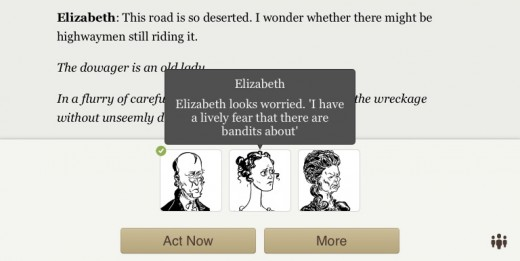
\includegraphics[width=.7\textwidth]{versu}
  \caption{An example of Versu's game play.}
  \label{fig:versu}
\end{figure}

The game is based upon two objects: agents and social practices.
Social practices describe a recurring social situation that may exist only for a short time (e.g. a conversation, a game, a meal) or can last much longer (e.g. a family, the moral community).
These practices coordinate agents via the \textit{roles} they are playing and their main function is to describe the actions the agents can do in each situation.

Social practices provide the agent with a set of suggested actions, but it is up to the agent himself to decide which action to perform, using utility-based reactive action selection (the utility is calculated in accordance with the agents beliefs, desires, personality quirks, and backstory).

Versu's world allows multiple practices to exist concurrently. For example, in a dinner party, there will be multiple practices operating at once:
\begin{itemize}
\item eating and drinking.
\item the conversation about politics
\item the rising flirtation between Frank and Lucy
\item responding to the fact that Mr. Quinn has spilled the soup.
\end{itemize}

Performing an action can result in any sentence being added to the world database.
The results of adding new sentences can be that relationships are updated, new beliefs or desires are formed, old practices are deleted or new practices are spawned.

Agents and social practices are scripts authored in a high-level \ac{DSL} designed specifically for this simulation: Praxis\footnote{Praxis is based on Exclusion Logic \cite{evans:exclusion-logic}, a new deontic logic.}.

Versu's success is proof that the architecture can produce social agents with high adaptability.
But, as some of the already explored works, Versu's agents lack planning capabilities.
It's logic powered approach is a differentiating aspect from the previous models, however it does imposes some limitations.
One example is how the agents beliefs are expressed.
The system cannot represent universal and existential quantifiers (e.g. "everyone has become insane" and "the murderer is one of the guests", respectively) or beliefs about others' beliefs (e.g. "Mr Quinn believes that Lucy believes that Mrs Quinn is the murderer").
